\documentclass{article}
\usepackage{amsmath}
\usepackage{amssymb}
\newcommand*{\qed}{\hfill\ensuremath{\blacksquare}}
\usepackage{graphicx}
\graphicspath{{.}}
\usepackage{hyperref}
\usepackage{tikz}
\usepackage{pgfplots}
\long\def\/*#1*/{}
\usetikzlibrary{arrows}
\newcommand\tab[1][1cm]{\hspace*{#1}}


\title{Computational Linear Algebra, Module 11}
\author{Maya Shende}
\date{Due: April 18th, 2018}

\begin{document}
\maketitle

\begin{enumerate}

%exercise 1
\item output:\\
\begin{tabular}{cc}
	$u=(0,1)$: & $u=(1,2)$:\\ 
	\includegraphics[scale=.3]{exercise1_a} & \includegraphics[scale=.3]{exercise1_b}\\
	$u=(1,0)$: & $u=(1,0)$ and $\textbf{A}[0][0] = -5$:\\ 
	\includegraphics[scale=.3]{exercise1_c} & \includegraphics[scale=.3]{exercise1_d}\\
\end{tabular}

%exercise 2
\item output:\\
	\begin{tabular}{ccc}
		$u=(1,1)$: & $u=(0,1)$: & $u=(0.1,1)$: \\ 
		\includegraphics[scale=.3]{exercise2_a} & \includegraphics[scale=.3]{exercise2_b} & \includegraphics[scale=.3]{exercise2_c}\\
		$u=(1,2)$: & $u=(1.1,2)$: & $u=(1.01,2)$: \\
		\includegraphics[scale=.3]{exercise2_d} & \includegraphics[scale=.3]{exercise2_e} & \includegraphics[scale=.3]{exercise2_f}\\
	\end{tabular}

%exercise 3
\item 	$$ \begin{bmatrix}5 & -2 \\ 0 & 1\end{bmatrix} \begin{bmatrix}1 \\ 2\end{bmatrix} = \begin{bmatrix}1 \\ 2\end{bmatrix} = 1 \begin{bmatrix}1 \\ 2\end{bmatrix} $$
	The eigenvalue is $\lambda = 1$.
	
%exercise 4
\item 	Let $\textbf{y} = -2\textbf{x}$ then, $-\frac{1}{2}\textbf{y} = \textbf{x}$. Plugging back into the original formula $\textbf{Ax} = \lambda\textbf{x}$ gives you:
	$$ \textbf{A}(-\frac{1}{2}\textbf{y}) = \lambda(-\frac{1}{2}\textbf{y}) $$
	$$ \textbf{A}(-\frac{1}{2}\textbf{y}) = (-\lambda\frac{1}{2})\textbf{y} $$

%exercise 5
\item output: \\
\includegraphics[scale=.3]{exercise5}

%exercise 6
\item
	$$ \textbf{A}\textbf{x}_1 = \begin{bmatrix} 2 & 1 \\ 1 & 2 \end{bmatrix} \begin{bmatrix} \frac{1}{\sqrt{2}} \\ \frac{1}{\sqrt{2}} \end{bmatrix} = \begin{bmatrix} \frac{3}{\sqrt{2}} \\ \frac{3}{\sqrt{2}} \end{bmatrix} = 3 \begin{bmatrix} \frac{1}{\sqrt{2}} \\ \frac{1}{\sqrt{2}} \end{bmatrix} $$
	
	$$ \textbf{A}\textbf{x}_2 = \begin{bmatrix} 2 & 1 \\ 1 & 2 \end{bmatrix} \begin{bmatrix} \frac{1}{\sqrt{2}} \\ -\frac{1}{\sqrt{2}} \end{bmatrix} = \begin{bmatrix} \frac{1}{\sqrt{2}} \\ -\frac{1}{\sqrt{2}} \end{bmatrix} = 1 \begin{bmatrix} \frac{1}{\sqrt{2}} \\ -\frac{1}{\sqrt{2}} \end{bmatrix} $$
	
%exercise 7
\item Let $x_i$ be an eigenvector of A. Then, by definition, $Ax_i = \lambda_ix_i$. Then, \\
$A^2x_i = A(Ax_i) = A(\lambda_ix_i) = A\lambda_ix_i = \lambda_i(Ax_i) = \lambda_i\lambda_ix_i = \lambda_i^2x_i$. Now, we can use this fact and assume that for all $n \leq k-1$, $A^nx_i = \lambda_i^nx_i$ to inductively prove this. So, we have\\
$A^kx_i = A(A^{k-1}x_i) = A(\lambda_i^{k-1}x_i) = \lambda_i^{k-1}(Ax_i) = \lambda_i^{k-1}\lambda_ix_i = \lambda_i^kx_i$. \qed

%exercise 8
\item $\lambda_2 < \lambda_1$, and so we can say that $\frac{\lambda_2}{\lambda_1} < 1$, and so if we raise any number less than 1 to a power that approaches infinity, the denominator will grow much faster than the numerator, thus approaching 0. 

%exercise 9
\item Console Output: \\
	0.9486832980505138 0.31622776601683794 \\
	0.9970544855015815 0.07669649888473705 \\
	0.9998740474835989 0.015871016626723796 \\
	0.9999948963838328 0.0031948718734307767 \\
	0.999999795331072 6.397951345688243E-4 \\
	0.9999999918090485 1.279918074758798E-4 \\
	0.9999999996723283 2.5599672315805973E-5 \\
	0.9999999999868928 5.119986892766448E-6 \\
	0.9999999999994756 1.023999475711732E-6 \\
	0.999999999999979 2.04799979028478E-7 \\\\
	lambda=4.999999590399874 \\\\
	$\textbf{A}^k\textbf{u}^{(0)} = $2.4414063E7 1.0 \\
	
	The two vectors are not the same. 

%exercise 10

\item 

	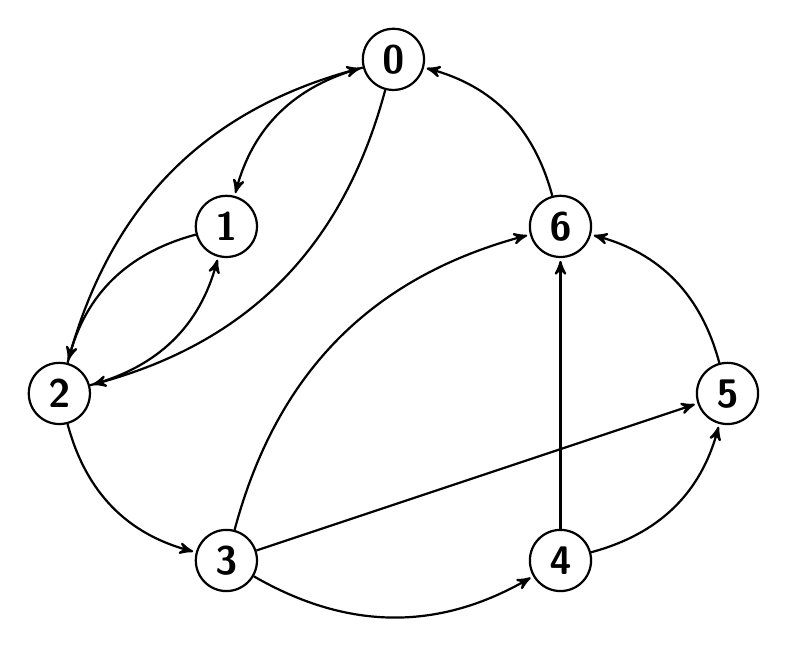
\begin{tikzpicture}[->,>=stealth',shorten >=1pt,auto,node distance=3cm,
	thick,main node/.style={circle,draw,font=\sffamily\Large\bfseries}]
	
	\node[main node] (1) {0};
	\node[main node] (2) [below left of=1] {1};
	\node[main node] (7) [below right of=1] {6};
	\node[main node] (3) [below left of=2] {2};
	\node[main node] (4) [below right of=3] {3};
	\node[main node] (6) [below right of=7] {5};
	\node[main node] (5) [below left of=6] {4};	
	
	\path[every node/.style={font=\sffamily\small}]
	(1) edge [bend left]  node[left] {} (3)
	edge [bend right] node[left] {} (2)
	(2) edge [bend right] node[left] {} (3)
	(3) edge [bend left]  node[left] {} (1)
	edge [bend right] node[left] {} (2)
	edge [bend right] node[left] {} (4)
	(4) edge [bend right] node[left] {} (5)
	edge              node[left] {} (6)
	edge [bend left]  node[left] {} (7)
	(5) edge [bend right] node[left] {} (6)
	edge              node[left] {} (7)
	(6) edge [bend right] node[left] {} (7)
	(7) edge [bend right] node[left] {} (1);
	
	\end{tikzpicture}
	\\\\
	$N(0) = \{(0,1), (0,2)\} $\\
	$N(1) = \{(1,2)\} $\\
	$N(2) = \{(2,0), (2,1), (2,3)\} $\\
	$N(3) = \{(3,4), (3,5), (3,6)\} $\\
	$N(4) = \{(4,5), (4,6)\} $\\
	$N(5) = \{(5,6)\} $\\
	$N(6) = \{(6,0)\} $
	\\
	

% exercise 11
\item \includegraphics[scale=.5]{exercise11}

%exercise 12
\item 
	$v_0(10) = 3 $\\
	$v_1(10) = 1 $\\
	$v_2(10) = 3 $\\
	$v_3(10) = 1 $\\
	$v_4(10) = 0 $\\
	$v_5(10) = 1 $\\
	$v_6(10) = 1 $

%exercise 13
\item 
	$\frac{v_0(t)}{t} = 0.1987$\\
	$\frac{v_1(t)}{t} = 0.2091$\\
	$\frac{v_2(t)}{t} = 0.3092$\\
	$\frac{v_3(t)}{t} = 0.0993$\\
	$\frac{v_4(t)}{t} = 0.0324$\\
	$\frac{v_5(t)}{t} = 0.0519$\\
	$\frac{v_6(t)}{t} = 0.0993$
	
%exercise 14
\item You find the subset of pages relevant to the search query by examining the probabilities of page as it relates to the current page or search term and then sort the different probabilities, $\pi_i$.

%exercise 15
\item 
	$$\textbf{P} = \begin{bmatrix} 
	0 & 0.5 & 0.5 & 0 & 0 & 0 & 0 \\ 
	0 & 0 & 1 & 0 & 0 & 0 & 0 \\
	0.33 & 0.33 & 0 & 0.33 & 0 & 0 & 0 \\
	0 & 0 & 0 & 0 & 0.33 & 0.33 & 0.33 \\
	0 & 0 & 0 & 0 & 0 & 0.5 & 0.5 \\
	0 & 0 & 0 & 0 & 0 & 0 & 1 \\
	1 & 0 & 0 & 0 & 0 & 0 & 0 \\ 
	\end{bmatrix}$$
	
	\includegraphics[scale=1]{exercise15}
	\\\\
	The relationship between the entries of the matrix and $N(i)$ is the entry in the matrix is zero unless there is an coordinate in the $N(i)$ and the value is the 1 divided by the size of the set $N(i)$.
	
%exercise 16
\item The eigenvalue for $\textbf{A}\pi = \pi$ is $1$.  

%exercise 17
\item They are roughly equal. \\
\includegraphics[scale=1]{exercise17}

%exercise 18
\item The matrix \textbf{P} is a probability matrix, where each row is the probability of transitioning between any other node and the node associated with that row. Therefore, the sum of all probabilities across a single row must equal 1. 

%exercise 19
\item 

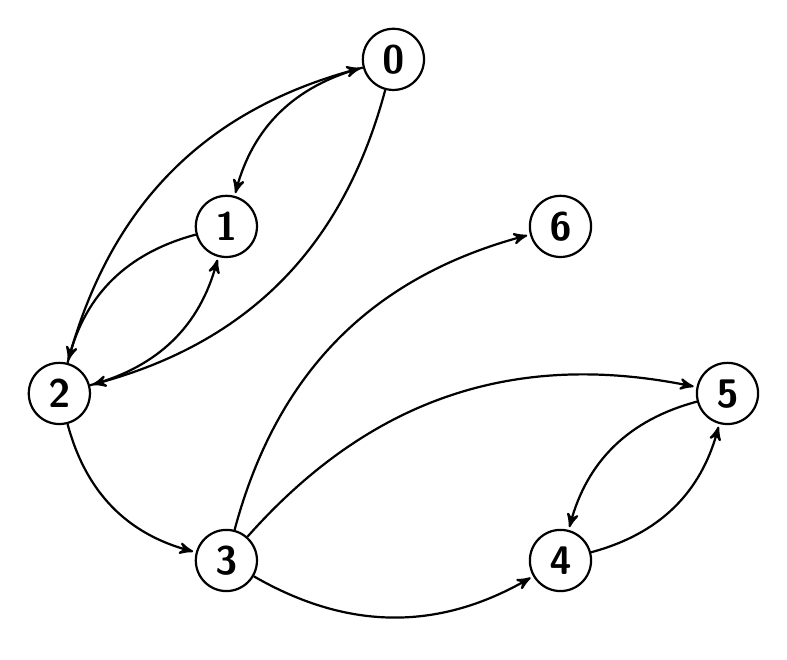
\begin{tikzpicture}[->,>=stealth',shorten >=1pt,auto,node distance=3cm,
	thick,main node/.style={circle,draw,font=\sffamily\Large\bfseries}]
	
	\node[main node] (1) {0};
	\node[main node] (2) [below left of=1] {1};
	\node[main node] (7) [below right of=1] {6};
	\node[main node] (3) [below left of=2] {2};
	\node[main node] (4) [below right of=3] {3};
	\node[main node] (6) [below right of=7] {5};
	\node[main node] (5) [below left of=6] {4};	
	
	\path[every node/.style={font=\sffamily\small}]
	(1) edge [bend left]  node[left] {} (3)
	edge [bend right] node[left] {} (2)
	(2) edge [bend right] node[left] {} (3)
	(3) edge [bend left]  node[left] {} (1)
	edge [bend right] node[left] {} (2)
	edge [bend right] node[left] {} (4)
	(4) edge [bend right] node[left] {} (5)
	edge [bend left] node[left] {} (6)
	edge [bend left]  node[left] {} (7)
	(5) edge [bend right] node[left] {} (6)
	(6) edge [bend right] node[left] {} (5);
	
	\end{tikzpicture}
	\\\\
	Node 6 does not link to anything and nodes 4 and 5 form an endless loop.


%exercise 20
\item

%exercise 21
\item It solves the dangling problem because now the surfer always has the option of jumping to a random node that may or may not have any links to any other nodes. 

%exercise 22
\item $ \frac{1}{n}hh^T = \frac{1}{n}
\begin{bmatrix}
1	&1	&1	&\dots	&1
\end{bmatrix}
\begin{bmatrix}
1\\
1\\
1\\
\vdots \\
1
\end{bmatrix}
= \frac{1}{n}
\begin{bmatrix}
1	&1	&\dots	&1\\
1	&1	&\dots	&1\\
\vdots	&\vdots	&\ddots	&\vdots \\
1	&1	&\dots	&1
\end{bmatrix}
= 
\begin{bmatrix}
 \frac{1}{n}	& \frac{1}{n}	&\dots	& \frac{1}{n}\\
 \frac{1}{n}	& \frac{1}{n}	&\dots	& \frac{1}{n}\\
\vdots	&\vdots	&\ddots	&\vdots \\
 \frac{1}{n}	& \frac{1}{n}	&\dots	& \frac{1}{n}
\end{bmatrix} $

%exercise 23
\item In the last step, we are basically just summing the terms in $x^{k-1}$ because $h^T$ is a row of 1's.\\
	We know
	$$\textbf{h}^T \textbf{x}^{(k-1)} = \begin{bmatrix} 1 & 1 & ... & 1 \end{bmatrix} \begin{bmatrix} p_1 \\ p_2 \\ \vdots \\ p_n \end{bmatrix}$$
	where $p_1 + p_2 + ... + p_n = 1$. From vector-vector multiplication, we get:
	$$  \begin{bmatrix} (1)p_1 + (1)p_2 + ... + (1)p_n \end{bmatrix} = 1$$ 

%exercise 24
\item It is sparse because it is a transition matrix, and we are not assuming that the graph is fully connected or mostly connected, therefore we call it sparse. 

%exercise 25
\item Pseudocode\\\\
	{\tt function: matrix-vector multiplication \{ \\
	\tab	Let u be the vector\\
	\tab	Let A be a collection of linked lists\\
	\tab	for each linked list in the collection: \\
	\tab\tab		for each entry in u, i:\\
	\tab\tab\tab		 result[i] += A.currentNode.getValue * u[i]\\
	\tab\tab\tab		 A.currentNode.getValue = A.getNextNode
			 \\
		\} }

%exercise 26
\item The eigenvalues were $\lambda = 3$ for $\textbf{x}_1$ and $\lambda = 1$ for $\textbf{x}_2$.
	\\\\
	\includegraphics[scale=1]{exercise26}


\end{enumerate}
\end{document}